\section{Einzelne Entscheidungsbäume}
\label{sec:construction}
\begin{figure}
    \centering
    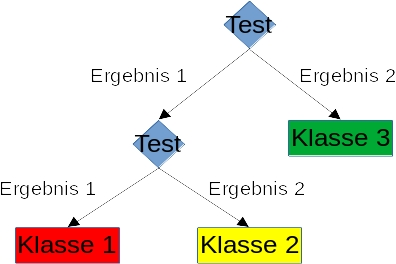
\includegraphics[width=0.5\linewidth]{images/entscheidungsbaum.jpg}
    \caption{Beispiel eines binären Entscheidungsbaums mit 3 möglichen Ergebnissen.}
    \label{fig:entscheidungsbaum}
\end{figure}
Der einzelne Entscheidungsbaum ist eine rekursive Datenstruktur um Entscheidungsregeln darzustellen. Jedem inneren Knoten ist ein \textit{Test} zugeordnet, der eine arbiträre Anzahl von sich gegenseitig
auschließenden Ergebnissen hat. Das Ergebnis bestimmt mit welchem Kindknoten fortgefahren wird \cite{quinlan1990decision}. Abbildung \ref{fig:entscheidungsbaum} zeigt einen Entscheidungsbaum, indem jeder Test
zwei mögliche Ergebnisse hat. Das wird als binärer Entscheidungsbaum bezeichnet.
\newline
\newline
Beim maschinellen Lernen werden aus mit Klassen beschrifteten Trainingsmengen Entscheidungsbäume generiert. Dabei wird die Trainingsmenge bestmöglich partitioniert, sodass die Blätter möglichst nur Einträge
enthält die mit der gleichen Klasse beschriftet sind. Dabei wird erhofft, dass der Entscheidungsbaum möglichst gut generalisieren kann, d. h. möglichst allgemeingültige Tests hat, die auf alle möglichen
Daten zutreffen und nicht nur auf die Trainingsmenge (TODO: Quelle).
\newline
\newline
Die Fähigkeit zu Generalisieren ist stark abhängig wie repräsentativ die Trainingsmenge ist und die Art und Weise, wie verschiedene Klassen in der Gesamtmenge unterschieden wird. Die Basis zum
Unterscheiden bieten sogenannte \textit{Feature}. Ein Feature kann ein Attribut sein oder eine berechnete Konsequenz aus mehreren Attributen der Rohdaten, z. B. der Durchschnitt oder das Maximum. Es ist
nicht aufgabe des Entscheidungsbaums aus den Rohdaten diese Feature zu extrahieren, sondern der Entscheidungsbaum nutzt eine vorgegebene Featuremenge die mit einer Klasse beschriftet ist (TODO: Quelle).
\newline
\newline
Es gibt verschiedene Algorithmen um Entscheidungsbäume zu erzeugen: \texttt{ID3}, \texttt{C4.5}, \texttt{C5}, \texttt{CART}, \texttt{CHAID}, \texttt{QUEST},
\texttt{GUIDE}, \texttt{CRUISE} and \texttt{CTREE} \cite{singh2014comparative}(TODO: Quellen für alle Algos im Detail). Das Grundprinzip der Partitionierung ist bei allen das Gleiche.
Sie unterscheiden sich aber in den verwendeten Metriken (TODO: Ist das wirklich so?).
\newline
\newline
In dieser Arbeit wird die Python ML-Bibliothek \textit{Scikit-Learn} verwendet. Sie implementiert eine optimierte Version des \texttt{CART} (Classification and Regression Trees) Algorithmus \cite{ScikitLearnCART}
und eine große Anzahl von Ensemble-Methoden \cite{scikit-learn}.
\newline
\newline
CART ist ein Greedy-Algorithmus, d. h. ein Algorithmus der lokal immer, auf basis einer Bewertungsfunktion, die beste Entscheidung wählt.
CART partitioniert die Trainingmenge und wählt dabei immer lokal die beste Teilung aus.
\begin{lstlisting}[label=lst:CARTtreeGrowing,caption={Skizze von vereinfachten Baumwachstumsalgorithmus \cite{steinbergCART}.}]
BEGIN:
Assign all training data to the root node
Define the root node as a terminal node

SPLIT:
New_splits=0
FOR every terminal node in the tree:
    If the terminal node sample size is too small or all instances in the node belong to the same target class goto GETNEXT
    Find the attribute that best separates the node into two child nodes using an allowable splitting rule
    New_splits+1

GETNEXT:
NEXT
\end{lstlisting}
Listing \ref{lst:CARTtreeGrowing} skizziert den vereinfachten Baumwachstumalgorithmus von CART. Der Algoritmus teilt die Trainingmenge solange, bis keine weitere Teilung mehr möglich ist oder alle Einträge der
mit der gleichen Klasse beschriftet sind. Folgend werden sukzessiv Teilbäume entfernt, die nach einer Bewertungsfunktion, z. B. Zuwachs der Erkennungsgenauigkeit, unterhalb eines vordefinierten
Schwellenwert liegen \cite{steinbergCART}.
\newline
\newline
Scikit-Learn bietet zusätzlich noch weitere Parameter an um die Konstruktion zu steuern, wie eine Maximalhöhe, Minimale Anzahl von Einträgen pro Blatt oder Teilung, oder daer minimale Anteil einer Klasse
um ein Blatt zu bilden \cite{ScikitLearnDTC}.